% ~~~~~~~~~~~~~~~~~~~~~~~~~~~~~~~~~~~~~~~~~~~~~~~~~~~~~~~~~~~~~~~~~~~~~~~~~~~~~
%                                 QUORIDOR
% ~~~~~~~~~~~~~~~~~~~~~~~~~~~~~~~~~~~~~~~~~~~~~~~~~~~~~~~~~~~~~~~~~~~~~~~~~~~~~
\chapter{Quoridor}\label{chap:3}
  \lhead{Chapter 3. \emph{Quoridor}}

\section{History}
\begin{wrapfigure}{R}{0.4\textwidth}
  \vspace*{-1.80cm}
  \centering
  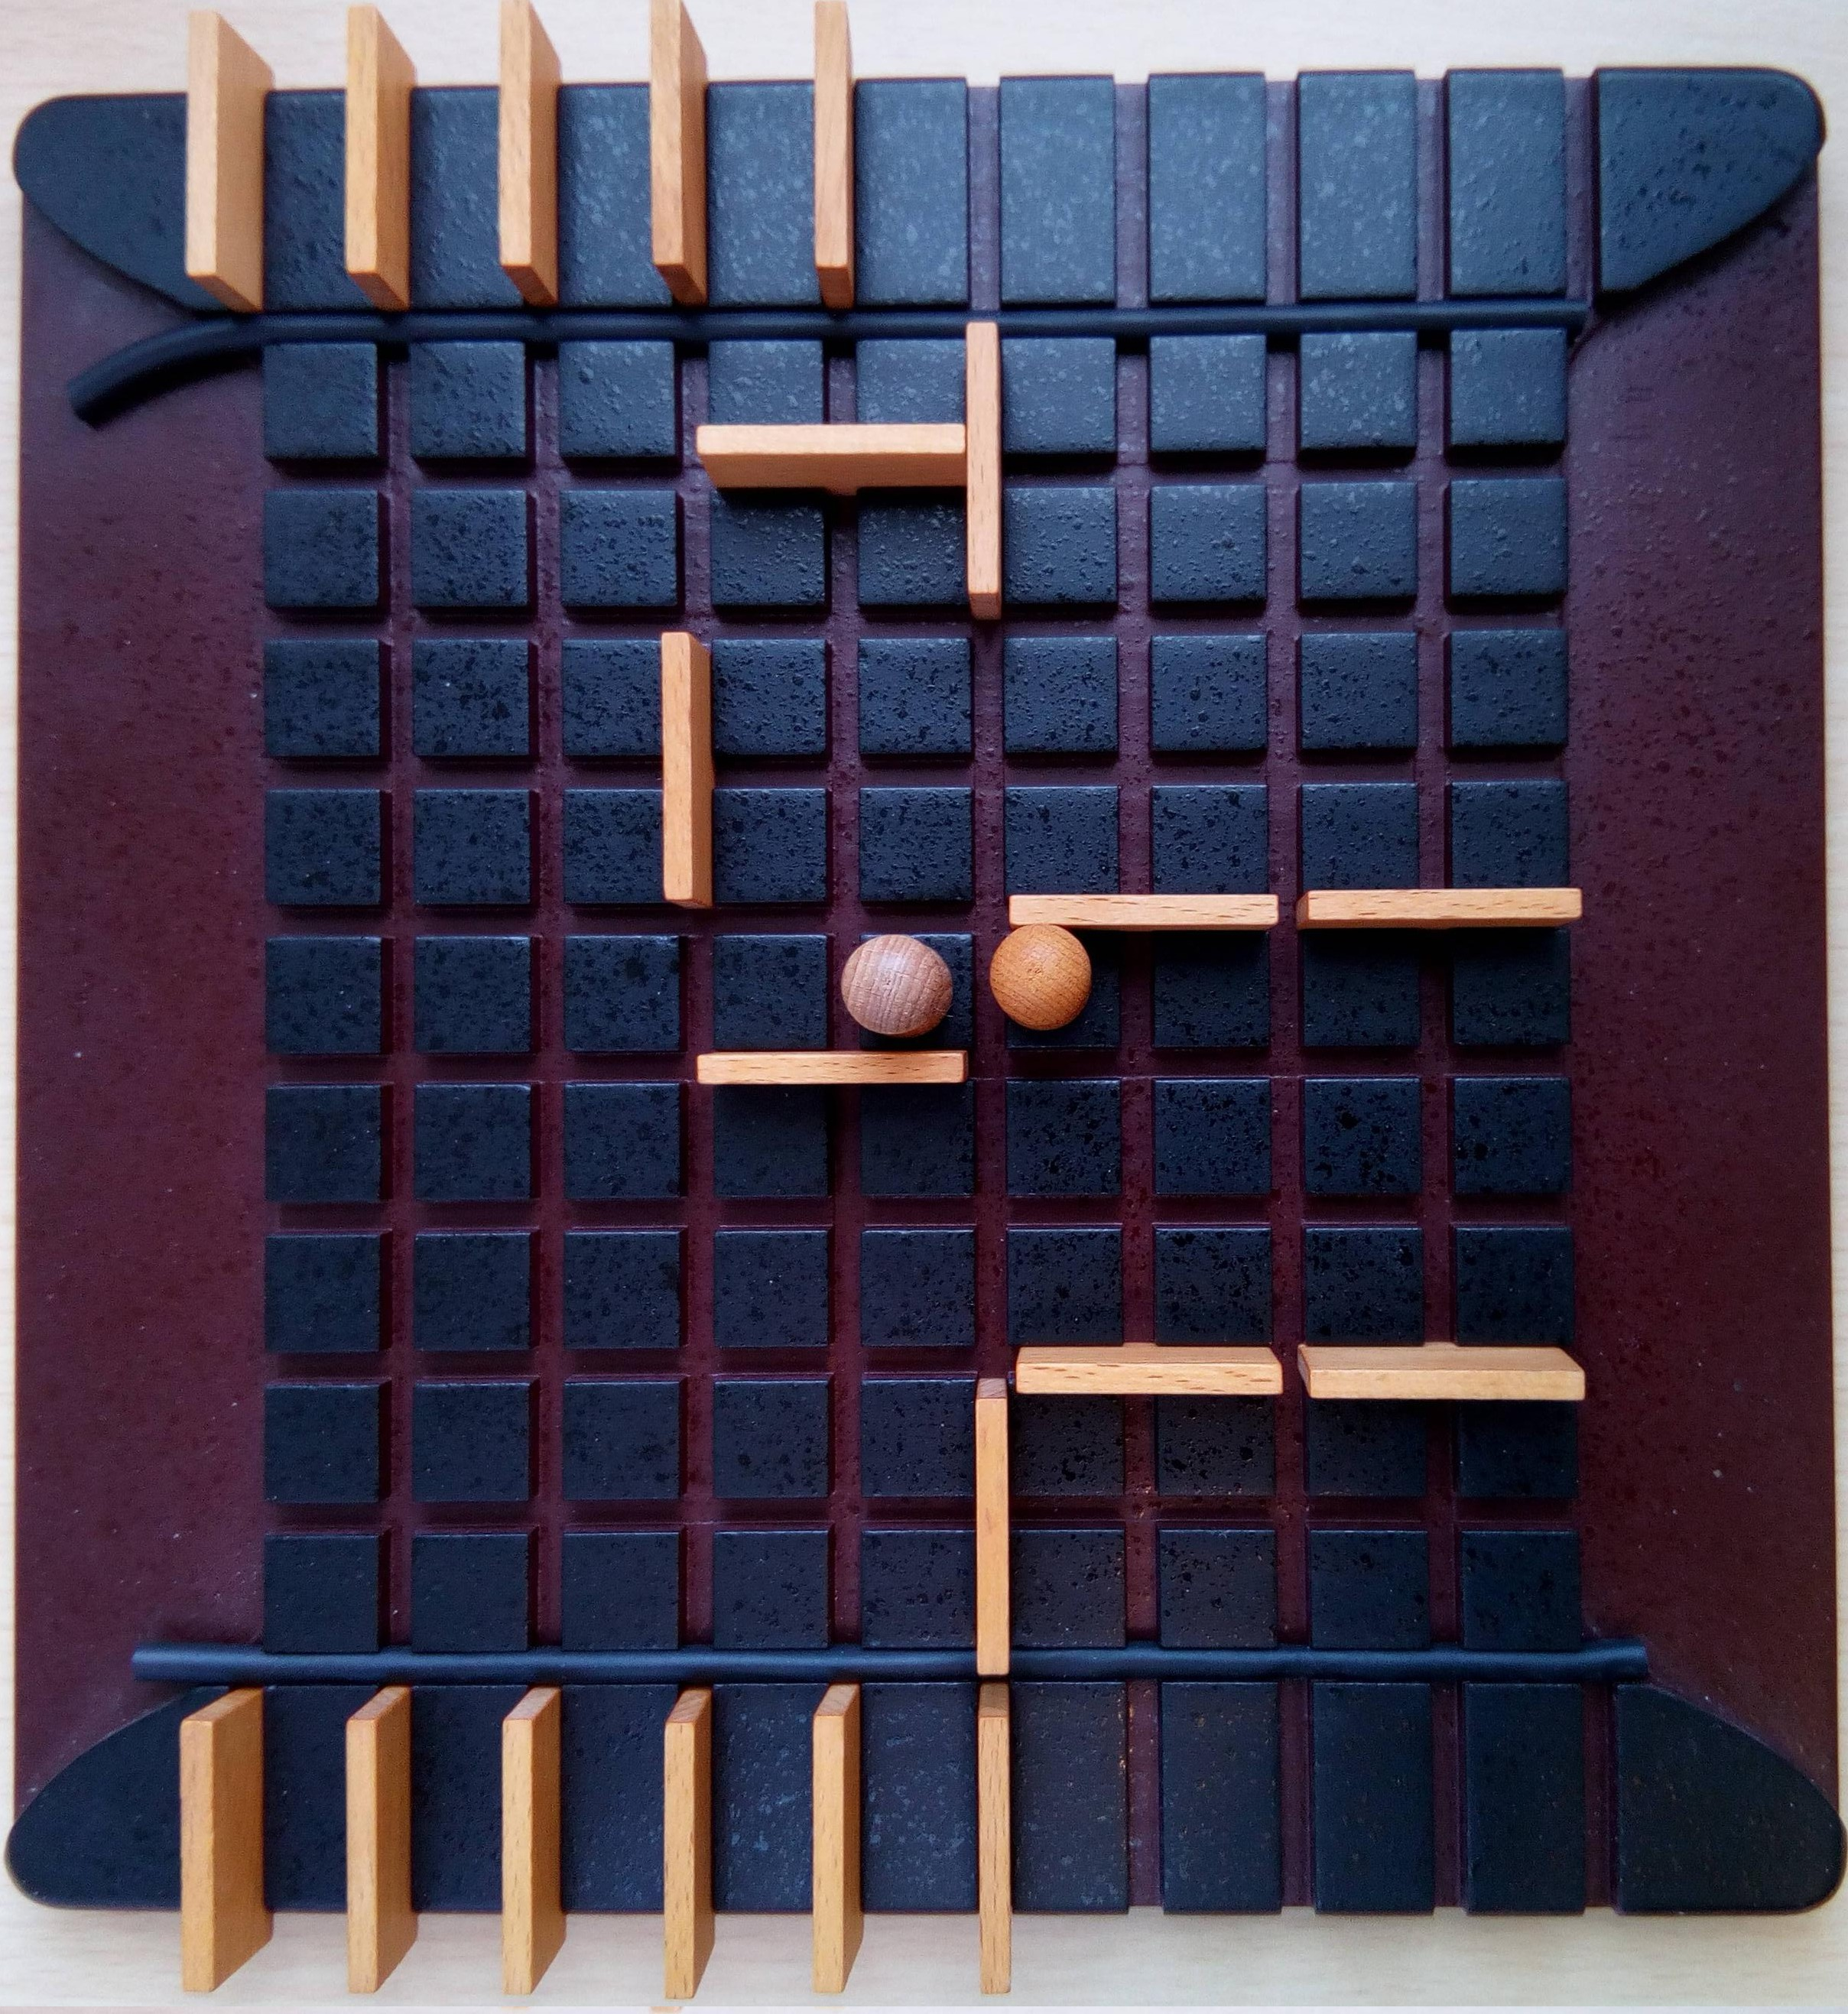
\includegraphics[width=0.35\textwidth]{real_board.jpg}
  \vspace*{-0.20cm}
  \caption{real board}
  \label{fig:quoridor_board}
  \vspace*{-1.40cm}
\end{wrapfigure}

Game Quoridor was invented by Mirko Marchesi based on game Blockade and
has been published by french company Gigamic Games in 1997. Since it has been
developed relatively early compared to other games such as Chess or Go, there
have been only few attempts of analysing the game and creating game agents.

\section{Rules}
Quoridor is abstract board strategy game for 2 or 4 players with size of
9x9 (81) squares. This thesis covers 2 player version of the game.

Each player starts with a single pawn in the center of the edge on the
opposite side as the opponent.
The goal for each player is to reach the opposite edge.

\begin{wrapfigure}{L}{0.35\textwidth}
  \vspace*{-0.60cm}
  \centering
  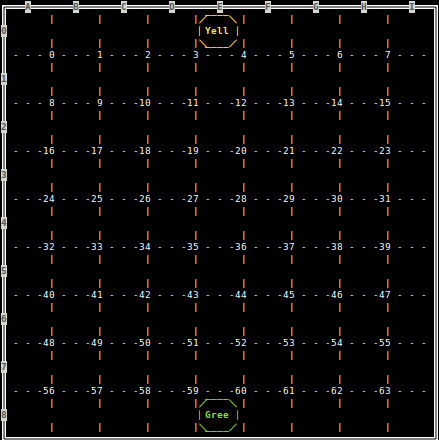
\includegraphics[width=0.35\textwidth]{start.png}
  \vspace*{-0.80cm}
  \label{fig:game_start}
  \caption{game start}
  \vspace*{-0.80cm}
\end{wrapfigure}

Player also starts with 10 walls (fences) in the stock.
Walls are two space wide and can be placed in the groove that runs between
the spaces.
Placed wall blocks pawns paths forcing them to go arount it.
Walls once placed can not be moved nor removed.
Wall can not be placed to the position already occupied or crossing by
other wall.
Also, wall can not cut off the only remaining path of any pawn to his goal.

When player is on turn, he must place wall, if he has left some, or move
his pawn to adjacent (not diagonal and unoccupied) space.
If opponent's pawn stands on an adjacent space, current player can jump
with his pawn to all the places where the opponent pawn can move.

\section{State Complexity}
Estimated game state complexity was $3.9905\cdot10^{42}$
\cite{mertens} (eq. \ref{eqn:mertensestimate}), however, this is very
rough estimate, since it includes many states multiple times where it counts
with permutations instead of combinations of walls.

\begin{center}
  \vspace*{-1.30cm}
  \begin{equation}
    \label{eqn:mertensestimate}
    \begin{aligned}
      S_p\!&=\!81 \cdot 80 = 6480 \\
      S_f\!&=\!\sum_{i=0}^{20}\prod_{j=0}^{i}(128 - 4i)\!=\!6.1582{\cdot}10^{38} \\
      S\!&=\!S_p \cdot S_f = \mathbf{3.9905 \cdot 10 ^{42}}
    \end{aligned}
  \end{equation}
  \vspace*{-1.15cm}
\end{center}

My approach (eq. \ref{eqn:myestimate}) with estimating state complexity
will be similar. I will estimate maximum states of this game, which will
include impossible states such as:
\begin{itemize}
  \vspace*{-0.25cm}
  \setlength\itemsep{0cm}
  \item walls crossing each other
  \item pawns in the winning position and on turn
  \item pawns not having the path to the winning position
  \item pawn in the winning position where it could not end due to walls
  \vspace*{-0.15cm}
\end{itemize}
Moreover, this estimate will differ between states when different
player is on the move, and also, when there is different number of walls
in players stocks. Both of these could make the game very different
in the outcome.

\begin{center}
  \vspace*{-1.30cm}
  \begin{equation}
    \label{eqn:myestimate}
    \begin{aligned}
      S_p &= 81 {\cdot} 80 - 9 {\cdot} 9 = 6399\\[-0.20cm]
      f(i)\!&=\! \begin{cases}
        i + 1  & \quad \text{if } i <= 10 \\[-0.30cm]
        21 - i & \quad \text{if } i > 10
      \end{cases}\\
      S_f\! &=\! \sum_{i=0}^{20} f(i){128 \choose i} = 1.7796 {\cdot} 10^{23}
      \\
      S &= 2 {\cdot} S_p {\cdot} S_f = \mathbf{2.2775{\cdot}10^{27}}
    \end{aligned}
  \end{equation}
  \vspace*{-1.15cm}
\end{center}

$S_p$ was corrected to not include both pawns in the winning positions.
$f(i)$ % is from sequence $\{1, 2, ..., 9, 10, 11, 10, 9, ..., 2, 1\}$ and
stands for different wall counts in the stocks.
${128 \choose i}$ are combinations of walls.
$2$ in $2{\cdot} S_p {\cdot} S_f$ represents different players on turn.

The result is maximum number of possible states, which is significantly
less then former estimate. However, even if I could evaluate $10^{6}$
states in one second, it would take around $7.2172{\cdot}10^{13}$ years to
evaluate this many states. Also, lets assume it takes on average 50B
of memory per state. Then I would need approximately
$1.1387{\cdot}10^{29}$ bytes of memory to store all states in the
computer. This is why simple Q-learning is not feasible.

\section{Game Tree Complexity}
Average branging factor of the game has been experimentaly measured to be
$60.4$ and average game length to be $91.1$ \cite{glendenning}.
Mertens \cite{mertens} used this to compute game-tree size $G$:
\begin{center}
  \vspace*{-1.30cm}
  \begin{equation}
    \label{eqn:mgtc}
    G = 60.4^{91.1} = 1.7884{\cdot}10^{162}
  \end{equation}
  \vspace*{-1.30cm}
\end{center}

\begin{wrapfigure}{r}{0.38\textwidth}
  \vspace*{-0.45cm}
  \centering
  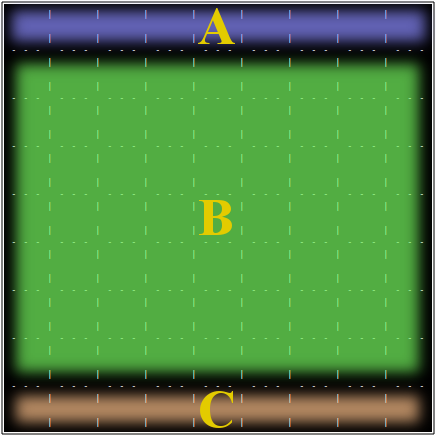
\includegraphics[width=0.35\textwidth]{areas.png}
  \vspace*{-0.30cm}
  \caption{board areas}
  \label{fig:areas}
  \vspace*{-0.60cm}
\end{wrapfigure}

To create my own estimate of branching factor, I will estimate number of states
where decision can be made and also number of different decisions possible. 
Branching factor will be simply division of these.

To count every possible pawn move, board is divided into three areas
(fig. \ref{fig:areas}), where $A$ and $C$ are positions from the first
and last row respectively and $B$ are positions from $7$ rows from the middle.
So, position AC means, first pawn is in the first row and second pawn is
in the last row or BB means, both pawns are in the middle $7$ rows. Then, for
each pattern (fig. \ref{fig:decisions}), possible positions for making
decision and possible decisions are counted.
% where $P$ represents number of possibilites and $D$ represents number of decisions possible.

\begin{wrapfigure}{H}{0.99\textwidth}
  \vspace*{-12.60cm}
  \centering
  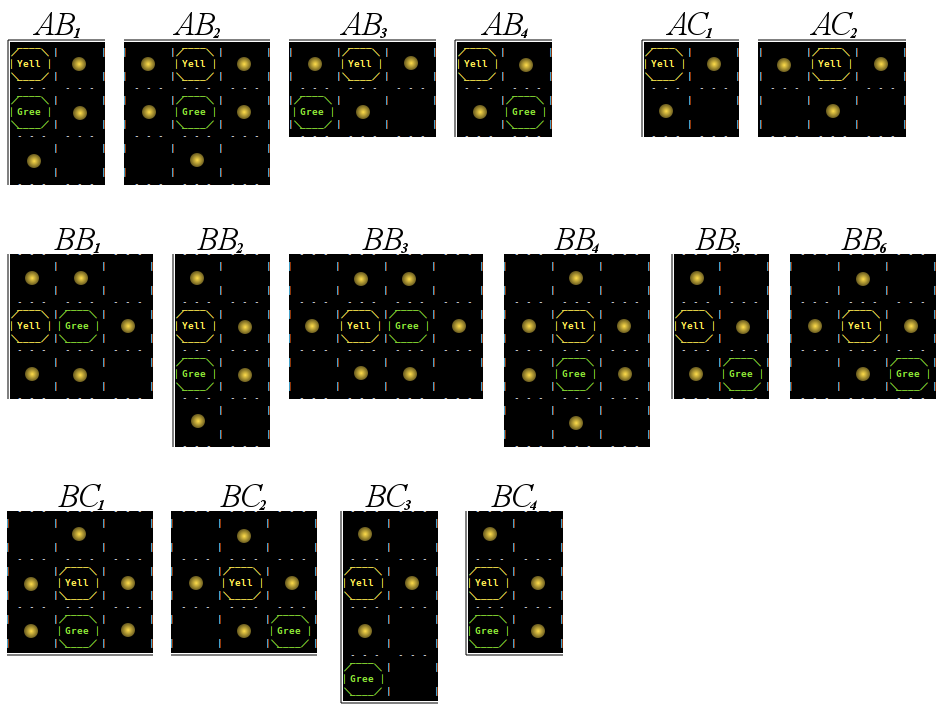
\includegraphics[width=0.95\textwidth]{decisions.png}
  \vspace*{-0.25cm}
  \caption{decision patterns}
  \label{fig:decisions}
  \vspace*{-0.60cm}
\end{wrapfigure}

\vspace{12.00cm}
\nobreakspace
In total, there are 3168 different positions where pawns can make decission and
from that, there are 11309 different decision that pawns can make
(see tab. \ref{tab:decisionstab}).
\newpage

\newcommand{\m}[2]{\multicolumn{1}{|#1}{#2}}
\newcommand{\rr}[6]{
  \m{l}{#1} & \m{r}{#2} & \m{r|}{#3} & & \m{l}{#4} & \m{r}{#5} & \m{r|}{#6} \\
}

\begin{table}[!h]
  \vspace*{0.2cm}
  \begin{tabular}{ l r r c l r r }
      \cline{2-3} \cline{6-7}
      & \m{c}{Positions} & \m{c|}{Decisions} & &
      & \m{c}{Positions} & \m{c|}{Decisions}
      \\ \cline{1-3} \cline{5-7}

      \rr{$AB_{1}$}{$2$}{$2{\cdot}3=6$}
         {$AC_{1}$}{$2{\cdot}9=18$}{$18{\cdot}2=36$}
         \cline{1-3} \cline{5-7}

      \rr{$AB_{2}$}{$7$}{$7{\cdot}5=35$}
         {$AC_{2}$}{$7{\cdot}9=63$}{$63{\cdot}3=189$}
         \cline{1-3} \cline{5-7}

      \rr{$AB_{3}$}{$7{\cdot}62=434$}{$434{\cdot}3=1302$}
         {$BB_{1}$}{$7{\cdot}2{\cdot}2=28$}{$28{\cdot}5=140$}
         \cline{1-3} \cline{5-7}

      \rr{$AB_{4}$}{$2{\cdot}62=124$}{$124{\cdot}2=248$}
         {$BB_{2}$}{$6{\cdot}2{\cdot}2=24$}{$24{\cdot}4=96$}
         \cline{1-3} \cline{5-7}

      \rr{$BC_{1}$}{$7$}{$7{\cdot}5=35$}
         {$BB_{3}$}{$6{\cdot}2{\cdot}7=84$}{$84{\cdot}6=504$}
         \cline{1-3} \cline{5-7}

      \rr{\multirow{2}{*}{$BC_{2}$}}
         {\multirow{2}{*}{%
           $\begin{matrix}42{\cdot}9{+}7{\cdot}8\\=434\end{matrix}$%
         }}%
         {\multirow{2}{*}{$434{\cdot}4=1736$}}
         {$BB_{4}$}{$6{\cdot}2{\cdot}7=84$}{$84{\cdot}6=504$}
         \cline{5-7}

      \rr{}
         {}
         {}
         {\multirow{2}{*}{$BB_{5}$}}
         {\multirow{2}{*}{%
           $\begin{matrix}%
             2{\cdot}2{\cdot}60{+}5{\cdot}2{\cdot}59\\%
             =830\\%
           \end{matrix}$%
         }}
         {\multirow{2}{*}{$830{\cdot}3=2490$}} \cline{1-3}

      \m{l}{\multirow{2}{*}{$BC_{3}$}} & \m{r}{\multirow{2}{*}{%
           $\begin{matrix}
             6{\cdot}9{\cdot}2{+}2{\cdot}8 \\
             = 124
           \end{matrix}$%
         }} & \m{r|}{\multirow{2}{*}{$124{\cdot}3=372$}}
      & &
      \m{l}{} & \m{r}{} & \m{r|}{} \\ \cline{5-7}

      \rr{}{}{}
         {\multirow{3}{*}{$BB_{6}$}}
             {\multirow{3}{*}{%
               $\begin{matrix}%
                 \displaystyle
                 {7{\cdot}9\choose2}{-}{\sum_{i<6}}BB_{i} \\
                 =903 \\
               \end{matrix}$%
             }}
             {\multirow{3}{*}{$903{\cdot}4=3612$}}
             \cline{1-3}

      \m{l}{$BC_{4}$} & \m{r}{$2$} & \m{r|}{$2{\cdot}2=4$} & & \m{l}{} & \m{r}{} & \m{r|}{} \\ \cline{1-3}
      & & & & \m{l}{} & \m{r}{} & \m{r|}{} \\ \cline{5-7}%

      % & & & & & & \\ \cline{4-6}%
      % & & & \multicolumn{2}{|r}{Positions} & \m{r|}{Decisions} & \\ \cline{3-6}%
      % & & \m{l}{\textbf{Total}} & \multicolumn{2}{|r}{$\textbf{3168}$} & \m{r|}{$\textbf{11309}$} & \\ \cline{3-6}%
  \end{tabular}
  \vspace*{0.20cm}
  \caption{positions and decisions}
  \label{tab:decisionstab}
  \vspace*{-0.30cm}
\end{table}

Next, maximum numbers of possible wall placement $N$ relative to walls already
placed $i$ are shown in table \ref{tab:placements}:
\begin{table}[!h]
  \vspace*{0.2cm}
  \begin{tabular}{r ccccccc ccccccc}
    \hline
    \m{r}{$i$} &
       \m{c}{0}  &   \m{c}{1} & \m{c}{2}   &   \m{c}{3} &   \m{c}{4} &
       \m{c}{5}  &   \m{c}{6} & \m{c}{7}   &   \m{c}{8} &   \m{c}{9} &
      \m{c}{10}  &  \m{c}{11} & \m{c}{12}  & \m{c|}{13} \\ \hline

    \m{r}{$N$} &
      \m{c}{128} & \m{c}{125} & \m{c}{123} & \m{c}{120} & \m{c}{118} &
      \m{c}{115} & \m{c}{113} & \m{c}{111} & \m{c}{109} & \m{c}{107} &
      \m{c}{105} & \m{c}{103} & \m{c}{101} & \m{c|}{98} \\ \hline

    & & & & & & & & & & & & & & \\ \cline{1-8}
    \m{r}{$i$} &
      \m{c}{14} & \m{c}{15} & \m{c}{16} & \m{c}{17} & \m{c}{18} & \m{c}{19} &
      \m{c|}{20} & & & & & & & \\ \cline{1-8}

    \m{r}{$N$} &
      \m{c}{96} & \m{c}{94} & \m{c}{92} & \m{c}{90} & \m{c}{88} & \m{c}{86} &
       \m{c|}{0} & & & & & & & \\ \cline{1-8}

  \end{tabular}
  \vspace*{0.20cm}
  \caption{wall placement possibilites}
  \label{tab:placements}
  \vspace*{-0.30cm}
\end{table}

\begin{wrapfigure}{R}{0.4\textwidth}
  \vspace*{-0.60cm}
  \centering
  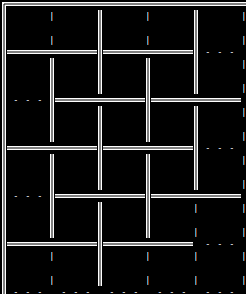
\includegraphics[width=0.35\textwidth]{tesselation.png}
  \vspace*{-0.20cm}
  \caption{min. tesselation example}
  \label{fig:mintess}
  \vspace*{-0.20cm}
\end{wrapfigure}

Optimal pattern for taking as least as possible from future wall placement
possibilities is shown in figure \ref{fig:mintess}. Naturally, placement starts
in the corner and the following walls are placed adjacent to each other.

Now, we can estimate all diferent states $S_d$ for making decision
(eq.  \ref{eqn:sestimate}), where $f(i)$ is the same function for stock factors
from equations \ref{eqn:myestimate}, ${128 \choose i}$ is top estimate
of different wall placement combinations.

Number of different decisions possible $D$ are sum of all possible
movemets and all possible wall placements. For wall placemnts
(eq. \ref{eqn:ge}), there are different stock factors $g(i)$, since state
where player moving has no walls in stock cannot place the wall.

\begin{equation}
  \label{eqn:ge}
  g(i) =
    \begin{cases}
      i + 1  & \quad \text{if } i <= 9 \\[-0.30cm]
      20 - i & \quad \text{if } i > 9
    \end{cases}\\
\end{equation}

\begin{equation}
  \label{eqn:sestimate}
  \begin{aligned}
    S_d &= 3168{\sum_{i=0}^{20}}{128 \choose i}f(i)
         = 5.6379{\cdot}10^{26} \\
    D &= {\sum_{i=0}^{20}}
         \left[
           11309f(i){128 \choose i}
           +
           3168g(i)N(i)){128 \choose i}
         \right]
       = 1.0766{\cdot}10^{28} \\
  \end{aligned}
\end{equation}

However, $S_d$ and $D$ include states where there are walls crossing each other and
pawns not having path to the winning position.
Moreover, $D$ does not count with number of movement possibilities taken
by placed walls.

\begin{equation}
  \label{eqn:brf}
  b = \frac{D}{S_d} = \frac{1.0766{\cdot}10^{28}}{5.6379{\cdot}10^{26}}
    = 19.0974
\end{equation}

The resulting estimate of branching factor $b$ is significantly lower than
the former estimate. But, it may be biased a little towards smaller number. It
would be caused by more combinations in situations with all walls placed having
more impossible possitions than the other.

Game tree complexity $C$ calculated with new branching factor estimate and
with former average game length:
\begin{equation}
  \label{eqn:gtc}
  C = 19.0974^{91.1} = \mathbf{4.9758{\cdot}10^{116}}
\end{equation}

